\documentclass[12pt,a4paper]{article}
\usepackage[utf8]{inputenc}
\usepackage[english]{babel}
\usepackage{enumerate}
\usepackage{amsmath}
\usepackage{amsfonts}
\usepackage{amssymb}
\usepackage{graphicx}
\usepackage{fourier}
\usepackage[left=2cm,right=2cm,top=2cm,bottom=2cm]{geometry}
\usepackage{commath}
\usepackage{cancel}
\usepackage{placeins}
\author{Juan Carlos Apitz, ID 012523821}
\title{STAT572 - Homework Assignment 9}
\begin{document}

\maketitle
\clearpage
\section*{Bayesian Inference with MCMC vs. Random Walk Sampler}

In this exercise we approximate the posterior distribution of the parameter $\theta$, which represents a hypothetical proportion of defective items in a sample of size $n=100$, generated by a Bernoulli process with $p=0.20$.\\

The left panel represents the distribution of the Markov Chain generated using Bayesian inference with MCMC. We use a
$\text{Unif}(0,1)$ as the prior and to calculate the transition probability use the likelihood function: \[L(\theta ,X)=\theta^{\sum x_i}(1-\theta)^{n-\sum x_i}\]
The right panel represents the Markov Chain generated using the Metropolis Random Walk sampler. In this case, the target distribution is proportional to the: \[\text{Beta}\bigr(\sum x_i+1,n-\sum x_i+1\bigr)\]
We sample using the random walk:
\[Y=X_t+\dfrac{Z_t}{\sqrt{12}}\] 
where \[Z_t=a+(b-a)u(0,1)\]
and $a=-0.5$, $b=0.5$. The result is that both processes generate random samples that follow a Beta distribution.

\begin{figure}[ht!] 
\begin{center}
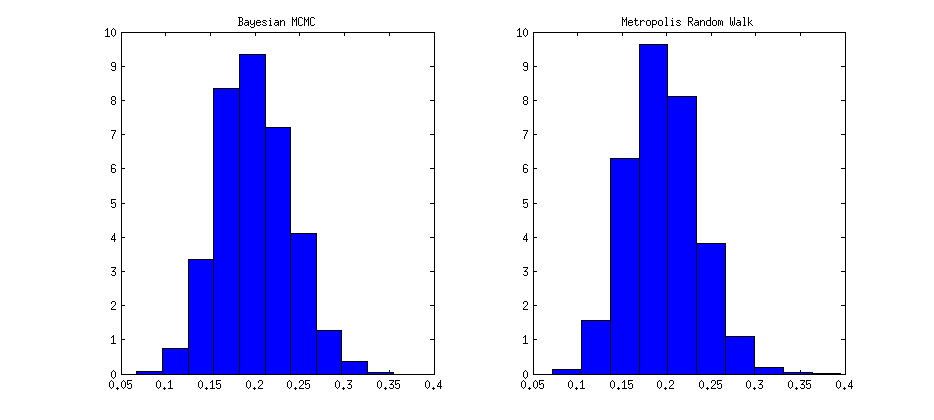
\includegraphics[scale=.7]{graph1.png}
\caption{The Markov Chain generated using the Bayesian approach represented by the graph on the left panel, has a mean $\bar{x}= 0.1993$ and a standard deviation $s=0.0402$. The Markov Chain generated using the Metropolis Random Walk sampler represented by the graph on the right panel, has a mean $\bar{x}=0.1959$ and a standard deviation $s=0.0393$. Note that the original data set used for this exercise was generated by a Bernoulli process with $p=0.20$, thus the results are expected.}
\label{inclass fig1}
\end{center}
\end{figure}
\FloatBarrier
\clearpage

\textbf{Mean \& Standard Deviation Results from MATLAB}
\begin{verbatim}
The mean of the Bayesian MC is: 0.1993

The std deviation of the Bayesian MC is: 0.0402

The mean of the Random Walk MC is: 0.1959

The std deviation of the Random Walk MC is: 0.0393
\end{verbatim}
\textbf{Code}
\begin{verbatim}
% PART 0. 
% generate hypothezied rs from bernoulli(0.2)
data = binornd(1,0.2,1,100); m = length(data);

% PART 1. 
% use the M-H sampler to generate MC of size 2000 whose invariance
% (target) distribution is given by the posterior distribution of
% theta|X

% Set up function handle to evaluate the likelihood.
likelihood = @(theta,x,n) theta.^sum(x).*(1-theta).^(n-sum(x));

% Generate 10000 samples in the chain.
n = 20000; % random sample size
% initialize the chain
mc1 = zeros(1,n);
mc1(1) = rand(1); % generate the starting point
for i = 2:n
    % generate a candidate from the chosen prior unif(0,1)
    y = unifrnd(0,1);
    % generate a uniform for comparison
    u = rand(1);
    alphaf = min([1, likelihood(y,data,m)/(likelihood(mc1(i-1),data,m))]);
    if u <= alphaf
        mc1(i) = y;
    else
        mc1(i) = mc1(i-1);
    end
end
% burn-in 5%
mc1= mc1(0.05*n+1:n);

% PART 2.
% Given that we know the posterior theta|x is dist Beta(sum(x)+1,n-sum(x)+1
% generate a MC from this dist using the random walk sampler.

% Set up function handle to evaluate the Beta kernel.
betapdfker = @(x,a,b) (x.^(a-1)).*((1-x).^(b-1));
alpha = sum(data)+1; beta = m-sum(data)+1; % parameters for the beata

% generate the MC
mc2 = zeros(1,n);
mc2(1) = rand(1); % generate the starting point
for i = 2:n
    % generate a candidate from the chosen prior unif(0,1)
    a = -0.5; b = 0.5;
    z = a + (b-a)*unifrnd(0,1);
    y = mc2(i-1)+z/sqrt(12);
    % generate a uniform for comparison
    u = rand(1);
    alphaf = min([1, betapdfker(y,alpha,beta)/(betapdfker(mc2(i-1),alpha,beta))]);
    if u <= alphaf
        mc2(i) = y;
    else
        mc2(i) = mc2(i-1);
    end
end
% burn-in 5%
mc2= mc2(0.05*n+1:n);

% Part 3.
% Calculate mean and sd
meanMC1 = mean(mc1);
stdMC1 = std(mc1);
meanMC2 = mean(mc2);
stdMC2 = std(mc2);
fprintf('\nThe mean of the Bayesian MC is: %2.4f\n',meanMC1)
fprintf('\nThe std deviation of the Bayesian MC is: %2.4f\n',stdMC1)
fprintf('\nThe mean of the Random Walk MC is: %2.4f\n',meanMC2)
fprintf('\nThe std deviation of the Random Walk MC is: %2.4f\n',stdMC2)

% Part 4.
% plot histograms and compare
figure(1)
subplot(1,2,1)
[fhath, bc] = hist(mc1);
fhath = fhath/((bc(2)-bc(1))*sum(fhath));
bar(bc,fhath,1,'b')
title('Bayesian MCMC')
subplot(1,2,2)
[fhath, bc] = hist(mc2);
fhath = fhath/((bc(2)-bc(1))*sum(fhath));
bar(bc,fhath,1,'b')
title('Metropolis Random Walk')
\end{verbatim}
\clearpage

\section*{Exercise 14.1}
The general von Mises pdf has the form:
\[f(x) = \dfrac{1}{2\pi I_0(b)}e^{b\cos(x-\mu)}\]
The parameter $\mu$ is the mean, so in this example we expect the mean of our sample to be close to zero. Additionally, our target distribution has the proportionality:
\[f(x|b)\propto e^{b\cos(x)}\]
Thus our algorithm uses the above relation to calculate $\alpha$, the transition probability, and $Y_t=X_t+Z_t$, where $Z_t\sim u(-1,1)$, as our random walk sampler. The generated Markov Chain and its histogram is shown in figure \ref{q1fig1} below.

\begin{figure}[ht!] 
\begin{center}
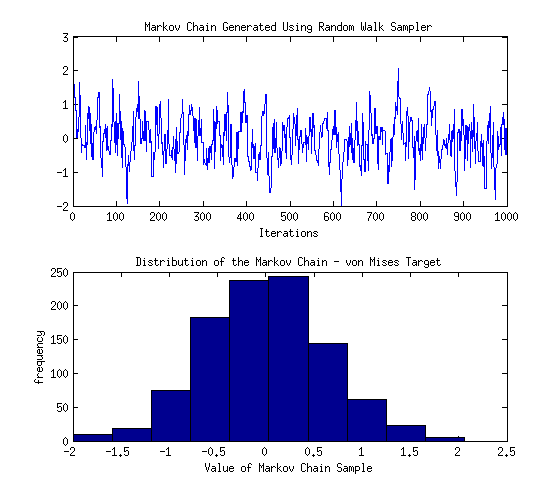
\includegraphics[scale=1]{graph2.png}
\caption{Markov Chain generated using the Metropolis Random Walk sampler (top panel) and histogram of the Markov Chain (bottom panel). Notice the random sample is centered at $\mu=0$.}
\label{q1fig1}
\end{center}
\end{figure}
\FloatBarrier

\textbf{Burn-In:} Since the starting point of the chain is 1, but our target distribution has a mean of zero, it would be advisable to "burn-in" the first few observations. That way, it is more likely that the chain obtained after the burn-in will be stationary and centered around the mean of the target distribution.Notice that the first few values start at about 1, and then converge towards zero.\\
\clearpage
\textbf{Code}
\begin{verbatim}
% Set up function handle to evaluate the von Mises kernel.
vonmisespdfker = @(x,b) exp(b.*cos(x));
b = 3; % parameters for the von mises

% generate the MC
n = 1000;
mc = zeros(1,n);
mc(1) = 2; % generate the starting point
for i = 2:n
    % generate a candidate from the random walk
    y = mc(i-1)+unifrnd(-1,1);
    % generate a uniform for comparison
    u = rand(1);
    alphaf = min([1, vonmisespdfker(y,b)/(vonmisespdfker(mc(i-1),b))]);
    if u <= alphaf
        mc(i) = y;
    else
        mc(i) = mc(i-1);
    end
end

% plots
figure(1)
subplot(2,1,1)
plot(mc) % entire MC
title('Markov Chain Generated Using Random Walk Sampler')
xlabel('Iterations')
subplot(2,1,2)
hist(mc)
title('Distribution of the Markov Chain - von Mises Target')
xlabel('Value of Markov Chain Sample')
ylabel('frequency')
\end{verbatim}
\clearpage

\section*{Exercise 14.2}
In this exercise we generate a random sample from the Beta$(0.5,0.5)$, the target distribution, using the Metropolis-Hastings algorithm. We sample candidates from the proposal distribution Unif$(\max(0, X_t-1),\min(1,X_t+1))$. The results in figure \ref{q2fig1} show that the sample generated closely resembles the density of the target distribution.
\begin{figure}[ht!] 
\begin{center}
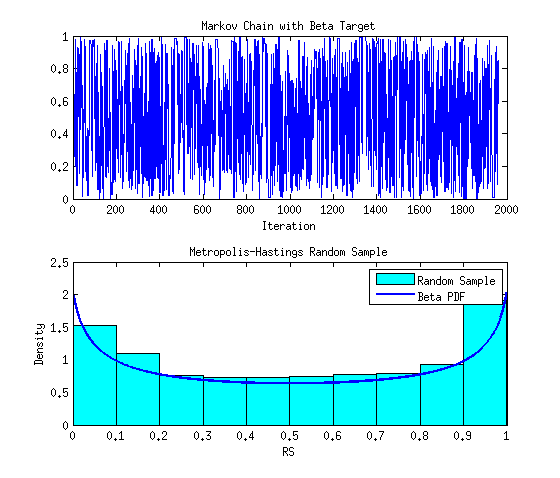
\includegraphics[scale=.9]{graph3.png}
\caption{Random sample generated using Metropolis-Hastings. \textbf{Proposal}: Unif$(\max(0, X_t-1,\min(1,X_t+1))$;  \textbf{Target}: Beta(0.5,0.5).}
\label{q2fig1}
\end{center}
\end{figure}
\FloatBarrier

\textbf{Code}
\begin{verbatim}
% METROPOLIS-HASTINGS TO GENERATE BETA SAMPLES

% Set up function handle to evaluate the Beta.
betapdfker = @(x,a,b) (x.^(a-1)).*((1-x).^(b-1));
a = 0.5; b = 0.5; % parameters for the beta
% set up function handle to evaluate the proposal distribution
unipdf = @(theta1,theta2) 1./(theta2-theta1);

% 1.GENERATE RANDOM SAMPLE OF SIZE n
% Generate 10000 samples in the chain.
n = 2000; % random sample size
% initialize the chain
x = zeros(1,n);
x(1) = rand(1); % generate the starting point
d = 1;
for i = 2:n
    % generate a candidate from the proposal distribution. This will be a
    % proposal with parameters given by the previous value in the chain.
    theta1 = max(0,x(i-1)-d);
    theta2 = min(x(i-1)+d,1);
    y = unifrnd(theta1,theta2,1,1);
    % generate a uniform for comparison
    u = rand(1);
    alphaf = min([1, betapdfker(y,a,b)*unipdf(y-d,y+d)/...
        (betapdfker(x(i-1),a,b)*unipdf(x(i-1)-d,x(i-1)+d))]);
    if u <= alphaf
        x(i) = y;
    else
        x(i) = x(i-1);
    end
end
% burn-in 2%
x= x(0.02*n+1:n);

% 2. PLOT THE RESULTS
subplot(211)
plot(x)
xlabel('Iteration')
title('Markov Chain with Beta Target', 'FontSize',14)
subplot(212)
[fhath, bc] = hist(x);
fhath = fhath/((bc(2)-bc(1))*sum(fhath));
bar(bc,fhath,1,'c')
hold on
linebetapdf = plot(linspace(0,1,5000),betapdf(linspace(0.025,0.975,5000),a,b),'b','LineWidth',2);
xlabel('RS')
ylabel('Density')
title('Metropolis-Hastings Random Sample', 'FontSize',14)
legend('Random Sample','Beta PDF')
hold off
\end{verbatim}
\clearpage

\section*{Exercise 14.3}
In this exercise we generate a random sample from the Gamma$(2,3)$, the target distribution, using the Metropolis-Hastings algorithm. We sample candidates from the proposal distribution Unif$(\max(0, X_t-5,X_t+5)$. The results in figure \ref{q3fig1} show that the sample generated closely resembles the density of the target distribution.

\begin{figure}[ht!] 
\begin{center}
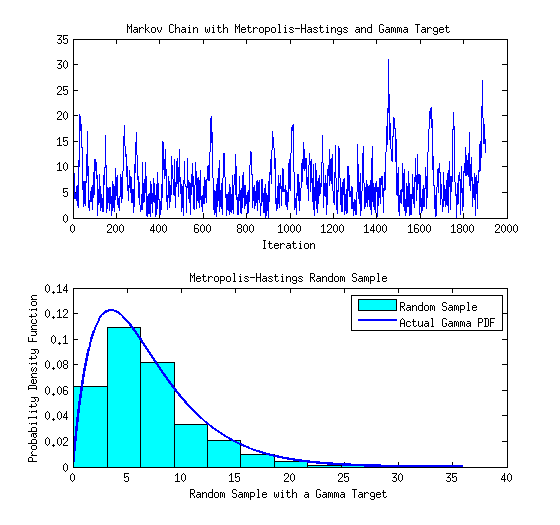
\includegraphics[scale=.95]{graph4.png}
\caption{Random sample generated using Metropolis-Hastings. \textbf{Proposal}: Unif$(\max(0, X_t-5,X_t+5)$;  \textbf{Target}: Gamma(2,3).}
\label{q3fig1}
\end{center}
\end{figure}
\FloatBarrier

\textbf{Code}
\begin{verbatim}
% METROPOLIS-HASTINGS

% Set up function handle to evaluate the gamma.
gammapdfker = @(x,a,b) (x.^(a-1)).*exp(-x./b);
a = 2; b = 3; % parameters for the gamma
% set up function handle to evaluate the proposal distribution
unipdf = @(theta1,theta2) 1./(theta2-theta1);

% 1.GENERATE RANDOM SAMPLE OF SIZE n
% Generate 20000 samples in the chain.
n = 2000; % random sample size
% initialize the chain
x = zeros(1,n);
x(1) = 1; %rand(1); % generate the starting point
d = 5;
for i = 2:n
    % generate a candidate from the proposal distribution. This will be a
    % proposal with parameters given by the previous value in the chain.
    theta1 = max(0,x(i-1)-d);
    theta2 = x(i-1)+d;
    y = unifrnd(theta1,theta2,1,1);
    % generate a uniform for comparison
    u = rand(1);
    alphaf = min([1, gammapdfker(y,a,b)*unipdf(y-d,y+d)/...
        (gammapdfker(x(i-1),a,b)*unipdf(x(i-1)-d,x(i-1)+d))]);
    if u <= alphaf
        x(i) = y;
    else
        x(i) = x(i-1);
    end
end
% burn-in 5%
x= x(0.05*n+1:n);

% 2. PLOT THE RESULTS
subplot(211)
plot(x)
xlabel('Iteration')
title('Markov Chain with Metropolis-Hastings and Gamma Target','FontSize',14)
subplot(212)
[fhath, bc] = hist(x);
fhath = fhath/((bc(2)-bc(1))*sum(fhath));
bar(bc,fhath,1,'c')
hold on
plot(linspace(0,max(x)+5,5000),gampdf(linspace(0,max(x),5000),a,b),'b','LineWidth',2);
xlabel('Random Sample with a Gamma Target')
ylabel('Probability Density Function')
title('Metropolis-Hastings Random Sample', 'FontSize',14)
legend('Metropolis Hasting Random Sample','Actual Gamma PDF')
hold off
\end{verbatim}
\clearpage
\section*{Exercise 14.4}
Figure \ref{q4fig1} below shows the random sample generated from the standard normal via Metropolis-Hastings with a chain starting value of 20 (which is very far from the actual mean of zero) and a burn-in rate of 2\%. Clearly, the sample is not quite adequate, having a denser upper tail, and not quite resembling the shape of the target distribution. We can also see, that it takes quite a few iterations for the chain to achieve stationarity around $\mu=0$.
\begin{figure}[ht!] 
\begin{center}
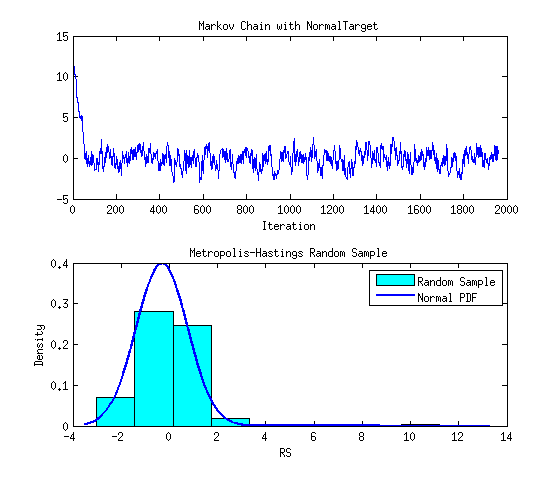
\includegraphics[scale=.95]{graph5.png}
\caption{Markov Chain/Random Sample from the standard normal. \textbf{Starting value}: 20, \textbf{burn-in}: rate 2\%. \textbf{Target}: Normal(0,1); \textbf{Proposal}: Unif$(X_t-1,X_t+1)$.}
\label{q4fig1}
\end{center}
\end{figure}
\FloatBarrier
\clearpage
Figure \ref{q4fig2} below shows a similarly generated random sample as in figure \ref{q4fig1} using the same starting value of 20 but now the burn-in rate is 20\%. Clearly, this sample is much more adequate adequate, closely resembling the shape of the target distribution. We can also see, that the chain is more or less stationary around $\mu=0$.
\begin{figure}[ht!] 
\begin{center}
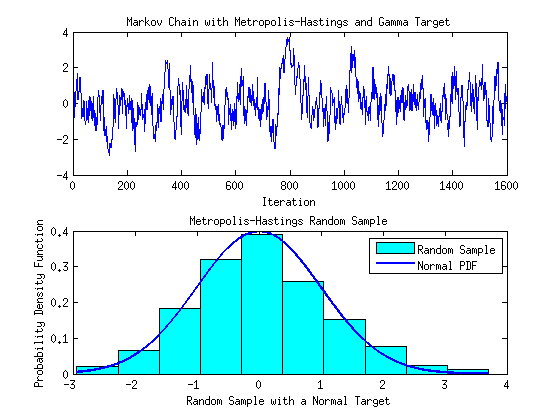
\includegraphics[scale=.95]{graph6.png}
\caption{Markov Chain/Random Sample from the standard normal. \textbf{Starting value}: 20, \textbf{burn-in rate}: 20\%. \textbf{Target}: Normal(0,1); \textbf{Proposal}: Unif$(X_t-1,X_t+1)$.}
\label{q4fig2}
\end{center}
\end{figure}
\FloatBarrier
\clearpage

Figure \ref{q4fig3} below shows a similarly generated random sample as in figure \ref{q4fig1} but using a starting value of 0 and a burn-in rate of 2\%. Clearly, this sample is adequate, closely resembling the shape of the target distribution. We can also see, that the chain is more or less stationary around $\mu=0$. In the case, since the chain starts close to its mean, we don't expect the burn-in rate to make much of a difference on an already adequate sample.
\begin{figure}[ht!] 
\begin{center}
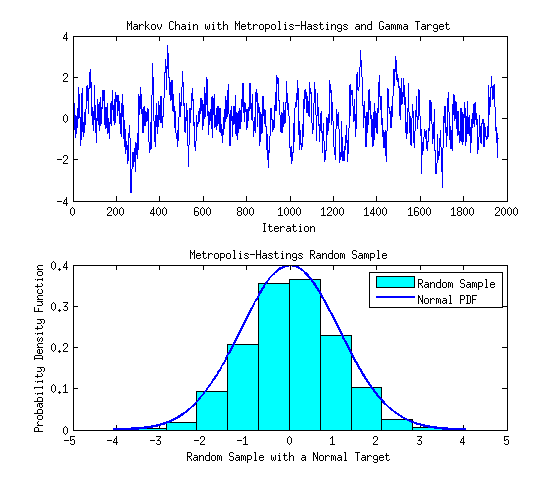
\includegraphics[scale=.95]{graph7.png}
\caption{Markov Chain/Random Sample from the standard normal. \textbf{Starting value}: 0, \textbf{burn-in rate}: 2\%. \textbf{Target}: Normal(0,1); \textbf{Proposal}: Unif$(X_t-1,X_t+1)$.}
\label{q4fig3}
\end{center}
\end{figure}
\FloatBarrier
\clearpage

Figure \ref{q4fig4} below shows a similarly generated random sample as in figure \ref{q4fig1} but using a starting value of 0 and a burn-in rate of 20\%. Clearly, this sample is  adequate, closely resembling the shape of the target distribution. We can also see, that the chain is more or less stationary around $\mu=0$. In the case, since the chain starts close to its mean, we confirm that the burn-in rate does not impact the adequacy of the sample generated given that the starting value of the chain is close to the mean of the target distribution.
\begin{figure}[ht!] 
\begin{center}
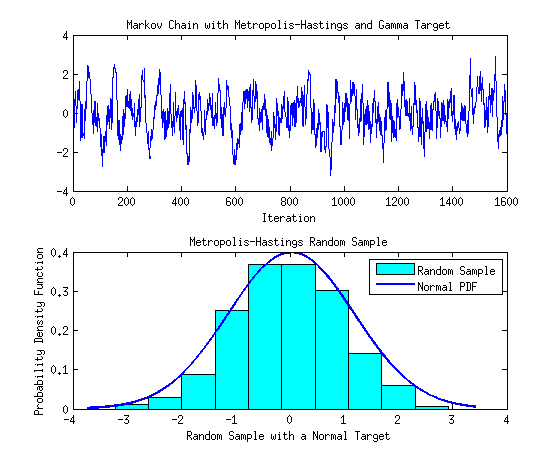
\includegraphics[scale=.95]{graph8.png}
\caption{Markov Chain/Random Sample from the standard normal. \textbf{Starting value}: 0, \textbf{burn-in rate}: 20\%. \textbf{Target}: Normal(0,1); \textbf{Proposal}: Unif$(X_t-1,X_t+1)$.}
\label{q4fig4}
\end{center}
\end{figure}
\FloatBarrier

\textbf{Code}
\begin{verbatim}
% METROPOLIS-HASTINGS

% Set up function handle to evaluate the target distribution.
normpdfker = @(x,mu,sigma) exp(-0.5*((x-mu)/sig).^2);
mu = 0; sig = 1; % parameters for the normal
% set up function handle to evaluate the proposal distribution
unipdf = @(theta1,theta2) 1./(theta2-theta1);

% 1.GENERATE RANDOM SAMPLE OF SIZE n
% Generate 20000 samples in the chain.
n = 2000; % random sample size
% initialize the chain
x = zeros(1,n);
x(1) = 20; %rand(1); % generate the starting point
for i = 2:n
    % generate a candidate from the proposal distribution. This will be a
    % proposal with parameters given by the previous value in the chain.
    theta1 = x(i-1)-1; theta2 = x(i-1)+1;
    y = unifrnd(theta1,theta2);
    % generate a uniform for comparison
    u = rand(1);
    alphaf = min([1, normpdfker(y,mu,sig)*unipdf(y-1,y+1)/...
        (normpdfker(x(i-1),mu,sig)*unipdf(x(i-1)-1,x(i-1)+1))]);
    if u <= alphaf
        x(i) = y;
    else
        x(i) = x(i-1);
    end
end
% burn-in 5%
x= x(0.02*n+1:n);

% 2. PLOT THE RESULTS
subplot(211)
plot(x)
xlabel('Iteration')
title('Markov Chain with Metropolis-Hastings and Gamma Target','FontSize',14)
subplot(212)
[fhath, bc] = hist(x);
fhath = fhath/((bc(2)-bc(1))*sum(fhath));
bar(bc,fhath,1,'c')
hold on
plot(linspace(min(x)-0.5,max(x)+0.5,5000),normpdf(linspace(min(x),max(x),5000),mu,sig),'b','LineWidth',2);
xlabel('Random Sample with a Normal Target')
ylabel('Probability Density Function')
title('Metropolis-Hastings Random Sample', 'FontSize',14)
legend('Random Sample','Normal PDF')
hold off
\end{verbatim}
\end{document}